\subsubsection{Combining TaskGenX with CATS}
\begin{figure*}[t]%
	\centering
	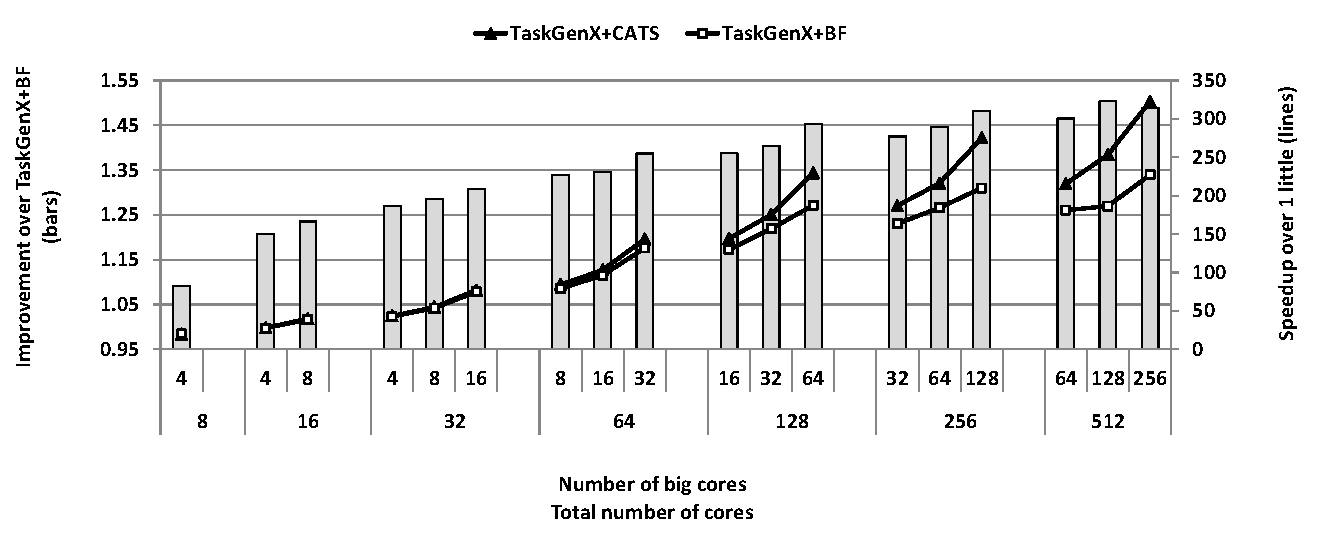
\includegraphics[width=\columnwidth]{figures/TaskGenX+CATS.pdf}
	\caption{Average speedup among 7 dependency synchronized workloads on heterogeneous simulated systems. The numbers at the bottom of x axis show the total number of cores and the numbers above them show the number of big cores.}	
	\label{fig:taskgenx_cats}
\end{figure*}
\begin{table*}[t]
	\begin{center}
		\caption{Evaluated benchmarks and relevant characteristics}
		\label{tab.taskgenx_cats}
		%\resizebox{\textwidth}{!}{%
		\begin{tabular}{|c|c|}
			\hline
			Workload & Avg improvement \\%& {\parbox{50mm}{\centering Per-task CREATE overheads (CPU cycles)}} \\
			\hline
			{\parbox{60mm}{\centering Cholesky 32K 256 (128$\times$128)}} & 0.3\% \\%& 24369 \\                                 
			\hline
			{\parbox{60mm}{\centering Cholesky 32K 128 (256$\times$256)}} & 0.8\% \\%& 31033  \\
			\hline
			{\parbox{60mm}{\centering Cholesky 16K 512 (32$\times$32)}} & 12\% \\%& 19133 \\
			\hline
			QR 16K 512 & 19\% \\%& 20109 \\
			\hline
			QR 16K 128 & 0.5\% \\%& 27620 \\
			\hline
			Bodytrack & 6\% \\%& 10009 \\ 
			%Heat diffusion & Heat &  &  &  &  &  & \\ 
			\hline
			Dedup & 335\% \\%& 1310  \\
			\hline 
			Ferret & 2\% \\%& 42429  \\
			\hline 
		\end{tabular}%}
	\end{center}
\end{table*}			
As shown in this section, TaskGenX effectively improves performance of asymmetric multi-core systems even if the scheduler used is not asymmetry-aware.
In this subsection we combine TaskGenX with the Criticality-Aware Task Scheduler (CATS) that was described in detail in Section~\ref{sec.scheduling.cats} and we comment on the improvements that CATS brings to the current TaskGenX approach.
CATS applies an effective scheduling policy that detects the critical tasks of the application and executes them on the fast cores of the system.
The critical tasks of an application are selected according to their inter-task dependencies. 
This makes CATS more suitable for applications that demonstrate intensive dependencies and TDGs that create long paths.
For applications that their parallelization is mostly based on data parallelism and do not have any inter-task dependencies a scheduler like CATS does not make much sense as it will schedule tasks as randomly as the default BF scheduler.
%In such cases there are no critical tasks, and all tasks are of the same importance since they can execute in parallel without the need of waiting for another task to finish.
For this reason, in this section we omit the results for applications that are barrier synchronized such as blackscholes, canneal, fluidanimate and streamcluster.
After performing experiments, we saw that these applications show no benefit by using CATS because CATS dynamically adapts to the application and gives similar schedules to BF\footnote{All tasks are of same priority so there is no distinction between critical and non-critical. Section~\ref{sec.scheduling.cats} provides detailed description of CATS and how it operates.}. 
Specifically, they present a slowdown around 2\% on average which is due to the task prioritization overhead of CATS.

Figure~\ref{fig:taskgenx_cats} shows the average improvement of TaskGenX+CATS over TaskGenX+BF in bars as well as their speedup in lines.
The average shown on Figure~\ref{fig:taskgenx_cats} is the average of the dependency-synchronized workloads used in this chapter which are: cholesky256, cholesky128, QR512, QR128, bodytrack, dedup and ferret.
As we can see, using an asymmetry-aware dynamic task scheduler on top of TaskGenX further improves the average performance of TaskGenX by up to 46\%.

Moving in more detail, Table~\ref{tab.taskgenx_cats} shows the average improvements obtained from each workload.
TaskGenX+CATS improves TaskGenX+BF by up to 2\% for the two cholesky workloads used here, with the average improvement being 0.3\%. 
%have an improvement from the use of CATS around 3\%. 
Even if cholesky is a dependency intensive application, the benefits of using CATS in combination with TaskGenX are not significant.
This is due to the fact that the specific inputs result at very wide TDGs in which the critical path is not as important.
To verify this fact, we have added the results from a narrow-TDG cholesky workload, which is the input of 16K with 512 block size.
With this workload TaskGenX+CATS achieves up to 22\% improvement over TaskGenX+BF.

The same behavior is observed with QR; the smaller the block size, the wider the TDG, leading to low impact of TaskGenX+CATS for the QR128 input.
TaskGenX+CATS bring improvements up to 61\% when increasing the block size of QR, with the QR512 input.

Bodytrack, Ferret and Dedup also benefit from the use of CATS.
Ferret exhibits high task creation overheads when using CATS, thus its benefit is limited.
TaskGenX compensates by accelerating these task generation overheads but still the improvement cannot surpass 12\% over TaskGenX+BF.
Dedup on the other hand shows very high benefits due to the efficient CATS scheduling.
Dedup is a very good candidate for schedulers like CATS as its TDG structure creates a long path of dependent tasks.
CATS manages to execute these tasks on the big cores resulting in improvements of up to 3.95$\times$.

%However, the dependency-synchronized workloads used in this section are not the ideal cases for CATS.
It is interesting to note that TaskGenX and CATS show somehow contradictory benefits depending on the workload granularity;
TaskGenX is more effective with fine-grained workloads of any synchronization type (barrier or dependency synchronization). 
CATS provides a more workload-specific solution as its performance highly depends on the TDG structure of the application.
However, when combined, TaskGenX and CATS achieve optimal results for asymmetric multi-core systems reaching up to 4$\times$ higher performance over the baseline (no TaskGenX) when the master thread runs on a little core and up to 1.95$\times$ higher performance when the master thread runs on a big core.
%Additionally, CATS benefits from more coarse-grained inputs in order to have the time to detect the new critical tasks while other tasks are being executed.
